%\title{LaTeX Portrait Poster Template}
%%%%%%%%%%%%%%%%%%%%%%%%%%%%%%%%%%%%%%%%%
% a0poster Portrait Poster
% LaTeX Template
% Version 1.0 (22/06/13)
%
% The a0poster class was created by:
% Gerlinde Kettl and Matthias Weiser (tex@kettl.de)
% 
% This template has been downloaded from:
% http://www.LaTeXTemplates.com
%
% License:
% CC BY-NC-SA 3.0 (http://creativecommons.org/licenses/by-nc-sa/3.0/)
%
%%%%%%%%%%%%%%%%%%%%%%%%%%%%%%%%%%%%%%%%%

%----------------------------------------------------------------------------------------
% PACKAGES AND OTHER DOCUMENT CONFIGURATIONS
%----------------------------------------------------------------------------------------

\documentclass[a0,portrait]{a0poster}
\usepackage[utf8]{inputenc}
\usepackage{algorithmic}

\usepackage{multicol} % This is so we can have multiple columns of text side-by-side
\columnsep=100pt % This is the amount of white space between the columns in the poster
\columnseprule=3pt % This is the thickness of the black line between the columns in the poster

\usepackage[svgnames]{xcolor} % Specify colors by their 'svgnames', for a full list of all colors available see here: http://www.latextemplates.com/svgnames-colors

\usepackage{empheq}
\usepackage[most]{tcolorbox}

\tcbset{colback=yellow!10!white, colframe=red!50!black, 
        highlight math style= {enhanced, %<-- needed for the ’remember’ options
            colframe=red,colback=red!10!white,boxsep=0pt}
        }

\definecolor{opticlimb}{rgb}{0,0.65,0.65}

%\usepackage{times} % Use the times font
%\usepackage{palatino} % Uncomment to use the Palatino font
%\usepackage{helvet}
\usepackage{tcolorbox}
\tcbuselibrary{theorems}

\newtcbtheorem[number within=section]{mytheo}{Theorem}%
{colback=blue!5,colframe=blue!35!black,fonttitle=\bfseries}{th}

\usepackage{avant}
\bibliographystyle{plainnat}
\usepackage{graphicx} % Required for including images
\graphicspath{{figures/}} % Location of the graphics files
\usepackage{booktabs} % Top and bottom rules for table
\usepackage[font=small,labelfont=bf]{caption} % Required for specifying captions to tables and figures
\usepackage{amsfonts, amsmath, amsthm, amssymb,bm} % For math fonts, symbols and environments
\usepackage{wrapfig} % Allows wrapping text around tables and figures
\usepackage{tikz}
\usepackage[T1]{fontenc}
\usepackage[utf8]{inputenc}
\usepackage[font=small,labelfont=bf,tableposition=top]{caption}
\usepackage[font=footnotesize]{subcaption}
\renewcommand{\familydefault}{\sfdefault}

\newcommand{\E}[1]{\mathbb{E}[#1]}
\newcommand{\parametre}[1]{\color{OrangeRed} #1 \color{Black}}
\newcommand{\etat}[1]{\color{ForestGreen} #1 \color{Black}}
\newcommand{\control}[1]{\color{Blue} #1 \color{Black}}
\DeclarePairedDelimiterX{\infdivx}[2]{(}{)}{%
  #1\;\delimsize\|\;#2%
}
\newcommand{\infdiv}{D_{KL}\infdivx}
%\newcommand{\donnee}[1]{\color{BurntOrange} #1 \color{Black}}
\newtheorem{thm}{Theorem}
\begin{document}

{\begin{tikzpicture}[remember picture, overlay]
     \node [anchor=north east, inner sep=8cm]  at (current page.north east)
     {
\includegraphics[height=5cm]{logo_x.jpg}
     
\includegraphics[height=5cm]{logo_inria.png}};
  \end{tikzpicture}}
%----------------------------------------------------------------------------------------
% POSTER HEADER 
%----------------------------------------------------------------------------------------

% The header is divided into two boxes:
% The first is 75% wide and houses the title, subtitle, names, university/organization and contact information
% The second is 25% wide and houses a logo for your university/organization or a photo of you
% The widths of these boxes can be easily edited to accommodate your content as you see fit

\begin{minipage}[b]{0.7\linewidth}
\veryHuge \color{Navy} \textbf{Fast Incremental Stochastic Version of the EM algorithm} \color{Black}\\[2cm] % Title
%\Huge\textit{Identification de système dynamique}\\[2cm] % Subtitle
\huge \textbf{B. Karimi$^{1,2}$, M. Lavielle$^{1,2}$, E. Moulines$^{2}$}\\[0.5cm] % Author(s)
\huge INRIA$^1$, CMAP École Polytechnique$^2$\\[0.4cm] % University/organization
\Large \texttt{belhal.karimi@polytechnique.edu}

\end{minipage}
%


\vspace{1cm} % A bit of extra whitespace between the header and poster content

%----------------------------------------------------------------------------------------

\begin{multicols}{2} % This is how many columns your poster will be broken into, a portrait poster is generally split into 2 columns

%----------------------------------------------------------------------------------------
% ABSTRACT
%----------------------------------------------------------------------------------------

%\color{Navy} % Navy color for the abstract

%\begin{abstract}
%\noindent The Expectation Maximization (EM), The Monte Carlo EM (MCEM) and the Stochastic Approximation EM (SAEM) are powerful inference algorithms in the context of missing data models. We introduce variants of those algorithms that justifies incremental versions where only one, or a batch of individuals, are considered at each iteration. Since Generalized EM framework can not be used in this case where the E-step is not computed exactly, we'll use the Generalized Alternative Minimization Framework to study the deterministic EM mapping in the context of continuous random variables and use this result for the different stochastic mappings considered under the constraint of selecting a single data at each iteration. In all those cases we'll prove almost-sure convergence and give experimental results on simple cases and on more complicated Pharmacokinetics models showing the effectiveness of our technique.
%\end{abstract}

%----------------------------------------------------------------------------------------
% INTRODUCTION
%----------------------------------------------------------------------------------------

%\color{SaddleBrown} % SaddleBrown color for the introduction
%\color{Navy} % Navy color
%\color{opticlimb}
\color{DarkSlateGray}

\section{Problem statement}
\color{Navy} % Navy color
%\color{DarkSlateGray} % DarkSlateGray color for the rest of the content
A wide class of statistical problems involves observed and unobserved data. We can consider, for example,
inverse problems concerning deconvolution, source separation, change-points detection, etc. Linear and nonlinear
mixed effects models can also be considered incomplete-data models. Estimation of the parameters of these
models is a difficult challenge. In particular, the likelihood of the observations cannot usually be maximized in
closed form. The EM algorithm proposed by Dempter, Laird and Rubin led to many variants when the conditional expectation of the complete log-likelihood is intractable. The MCEM (Meng, 1993) and the SAEM (Delyon, 1999) are two of them.\\
Following Neal, Hinton and Gunawardana efforts in justifying a variant version of the EM algorithm considering an incremental scheme, we decided to focus on the Incremental EM, MCEM and SAEM for continuous random variables.

%----------------------------------------------------------------------------------------
% OBJECTIVES
%----------------------------------------------------------------------------------------

\color{DarkSlateGray} % DarkSlateGray color for the rest of the content
%\vspace{1cm}
%\section{Model and notations}
%We study a classical missing data problem where:
%\begin{itemize}
%\item The observed data is a continuous random variable $Y = (Y_i, 1\leq i \leq N)$ that has observed values $(y_i, 1\leq i \leq N)$ in $\mathcal{Y}$
%\item The latent data is a continuous random variable $Z = (Z_i, 1\leq i \leq N)$ that takes on the values $(z_i, 1\leq i \leq N)$ in $\mathcal{Z}$ and consists in $N$ independent variables
%\item The components $Y_i$ are generated independently of each other and from their corresponding $Z_i$
%\item $\log p(y,\theta)$ is the incomplete data log-likelihood
%\item $\log p(y,z,\theta)$ is the complete data log-likelihood and obtained by augmenting the observed data with the missing data
%\item We'll call $P_{Y_i,Z_i,\theta}$ and $P_{Z_i|Y_i,\theta}$ the probability distributions associated to the densities $p(y_i,z_i,\theta)$ and $p(z_i|y_i,\theta)$
%\end{itemize}

%----------------------------------------------------------------------------------------
% MATERIALS AND METHODS
%----------------------------------------------------------------------------------------
%\vspace{1cm}
\section{Convergence Theorems}
   
\subsection{IEM algorithm}
Following Gunawardana work we can show that the IEM on missing data problem ($Y=(Y_i)_{i=1}^N$ are observed and $Z=(Z_i)_{i=1}^N$ are latent) can be seen as a Alternatively minimizing problem. In that context we proposed a criteria that we will be minimizing alternatively, for all $\theta \in \Theta$ and $(\delta_i)_{i=1}^N \in \Theta^N$:
\begin{align*}
  A \colon & \Theta^{N+1} \to \mathbb{R}\\
  & (\theta, \delta_1,\dots,\delta_N) \mapsto \infdiv{\prod_{i=1}^{N}{P_{Z_i|Y_i,\delta_i}}}{\prod_{i=1}^{N}{P_{Z_i|Y_i,\theta}}} - \sum_{i=1}^{N}{\log p(y_i,\theta)}
\end{align*}

Two successive mappings $ F_{I_k} \colon \Theta^{N+1} \to \Theta^{N+1}$, where $I_k$ is the index picked at iteration $k$, and $ B \colon \Theta^{N+1} \to \Theta^{N+1}$ decrease this criteria, strictly when the input is outside the solution set.
\begin{align*}
& F_{I_k}(\theta,\delta_{I_k},\delta_{-I_k}) = (\theta,\arg \min \limits_{\delta_{I_k} \in \Theta}  \infdiv{P_{z_{I_{k}}|y_{I_{k}},\delta_{I_k}}}{P_{z_{I_{k}}|y_{I_{k}},\theta^{k-1}}},\delta_{-I_k})\\
& B(\theta,(\delta_i)_{i=1}^N) = (\arg \min\limits_{\theta \in \Theta}A(\theta,\delta_1^{(k)},\dots, \delta_N^{(k)}),(\delta_i)_{i=1}^N)
\end{align*}
Using Zangwill global convergence theorem allows us to write this first convergence theorem.

Let $\{(\theta^k, \delta_1^k,\dots, \delta_N^k)\}_{k=0}^{\infty}$ be a sequence generated from a tuple $(\theta^0, \delta_1^0,\dots, \delta_N^0)$ by the iterative application, with its associated solution set $\Gamma$, of the point-to-set map $T = T_{1}\circ \dots \circ T_{N}$, where $T_{i} = B \circ F_{i}$ at each iteration $k$:
\begin{equation*}
(\theta^k, \delta_1^k,\dots, \delta_N^k) = T(\theta^{k-1}, \delta_1^{k-1},\dots, \delta_N^{k-1})
\end{equation*}


\begin{mytheo}{IEM convergence theorem}{theoexample}

Let $T: \Theta^{N+1} \to \Theta^{N+1}$ be the composition of the point-to-set maps $B$ and $F_{i}$ as defined in the algorithm.\\
With certain assumptions of compactness and continuity:
\begin{enumerate}
\item All accumulation points of the sequence $\{(\theta^k, \delta_1^k,\dots, \delta_N^k)\}_{k=0}^{\infty}$ lie in the solution set $\Gamma$
\item The sequence $\{\theta_k\}_{k=0}^{\infty}$ converges to stationary points of the incomplete data likelihood, i.e. all the accumulation points of this sequence are in  $\mathcal{L} = \{\theta \in \Theta, \partial_{\theta}l(\theta) = 0 \}$
\end{enumerate}

\end{mytheo}



\subsection{IMCEM algorithm}
One important assumption is needed in order to use the deterministic mapping $T$ to prove the convergence of the stochastic one $P_{k}$. For all $(\theta_k, \delta_1^k,\dots,\delta_N^k) \in \Theta^{N+1}$, $w.p.1$ :
\begin{equation*}
\lim\limits_{k} |A \circ P_{k}(\theta_k, \delta_1^k,\dots,\delta_N^k) - A \circ T(\theta_k, \delta_1^k,\dots,\delta_N^k)| = 0
\end{equation*}

 \begin{mytheo}{IMCEM convergence theorem}{imcem}
With certain assumptions of compactness and continuity and a sequence of parameter estimates $\{\theta_{k}\}$ satisfying the IMCEM algorithm:
\begin{enumerate}
  \item if $A(\mathcal{L}\cap\Theta,\dots,\mathcal{L}\cap\Theta)$ has an empty interior, then the accumulation points of $\{\theta_{k}\}_{k \geq 0}$ are in $\mathcal{L}$
\end{enumerate}
\end{mytheo}
   
   
   
\section{Incremental Algorithms in Practice}
\subsection{IMCEM on a simple Gaussian case}
Let's consider the case when all the variables of interest are Gaussian.
\begin{equation*}
Y_i = Z_i + \epsilon_i
\end{equation*}
Where $Z_i \sim \mathcal{N}(\theta,\omega^2)$ and $\epsilon_i \sim \mathcal{N}(0,\sigma^2)$.
Since the $Z_i$ and $\epsilon_i$ are i.i.d we have that $Y_i \sim \mathcal{N}(\theta,\sigma^2 + \omega^2)$ and $Y_i|Z_i \sim \mathcal{N}(Z_i,\sigma^2)$.\\
The goal is to find an estimate of the mean $\theta$ that maximizes the likelihood $p(y,\theta)$ considering that $\sigma^2$ and $\epsilon^2$ are known.

\noindent We can now apply our maximization step:
\begin{equation*}
\begin{split}
& \theta_{N+j} = \hat{\Theta}(S) = \frac{\alpha}{N} \sum_{i=1}^{N}{\theta_{N+j-i}} + (1-\alpha)\bar{y} + \bar{e}_{N+j}\\
\end{split}
\end{equation*}
Where $\bar{e} \sim \mathcal{N}(0, \frac{\gamma^2}{M_{N+j}N})$

If we define the vector of parameter as follow (with $k=N+j$):

\begin{equation*}
\theta_{k} = 
\left(
\begin{array}{c}
\theta_{k}\\
..\\
\theta_{k-N+1}\\
\end{array}
\right) = \rho \theta_{k-1} + (1-\alpha)\bar{y}e_1 + \bar{e}_k e_1
\textrm{  where  } \rho = \begin{pmatrix} 
\frac{\alpha}{N} & .. & .. & \frac{\alpha}{N} \\
1 & 0 & .. & 0\\
0 & 1 & .. & 0\\
.. & .. & .. & ..\\
.. & .. & .. & 0\\
\end{pmatrix}
\end{equation*}


\noindent Now if we consider a scheme where not only one individual is picked at each iteration but a batch pN (where p is a percentage). In that case we can write in scalar (to facilitate the notation we'll consider M=1 and $\bar{y} = 0$):
\begin{equation*}
\begin{split}
\theta_k & = \rho^{1/p} \theta_{k-1/p} + \frac{1-\rho^{1/p}}{1-\rho}\bar{e}_k
\end{split}
\end{equation*}
In that case we can calculate the expectation and the variance of our estimator $\theta_k$ in the stationary regime:

\begin{tcolorbox}[ams gather]
 \E{\theta_{k}} = \rho^{k/p}\theta_0\\
\textrm{Var } \theta_k = \frac{\gamma^2}{N(1-\rho)^2}\frac{1-\rho^{1/p}}{1+\rho^{1/p}}
\end{tcolorbox}
 


With these two expressions we understand what strategy is best for the choice of the batch size at each iteration. Indeed the bias is small when p is small so one should start with picking one individual first to kill the bias and the variance is decreasing when p is increasing. So once the bias is killed one should increase the size of the batch to kill the variance of the estimator.\\
\\
This result implies as well that the Online EM algorithm introduced by (Cappe and Moulines, 2007) is the best strategy to follow even when all the data is initially available. In other words, even though one has access to the whole observed dataset, one should consider increasing batch of individuals at each iteration.


\begin{center}%\vspace{1cm}
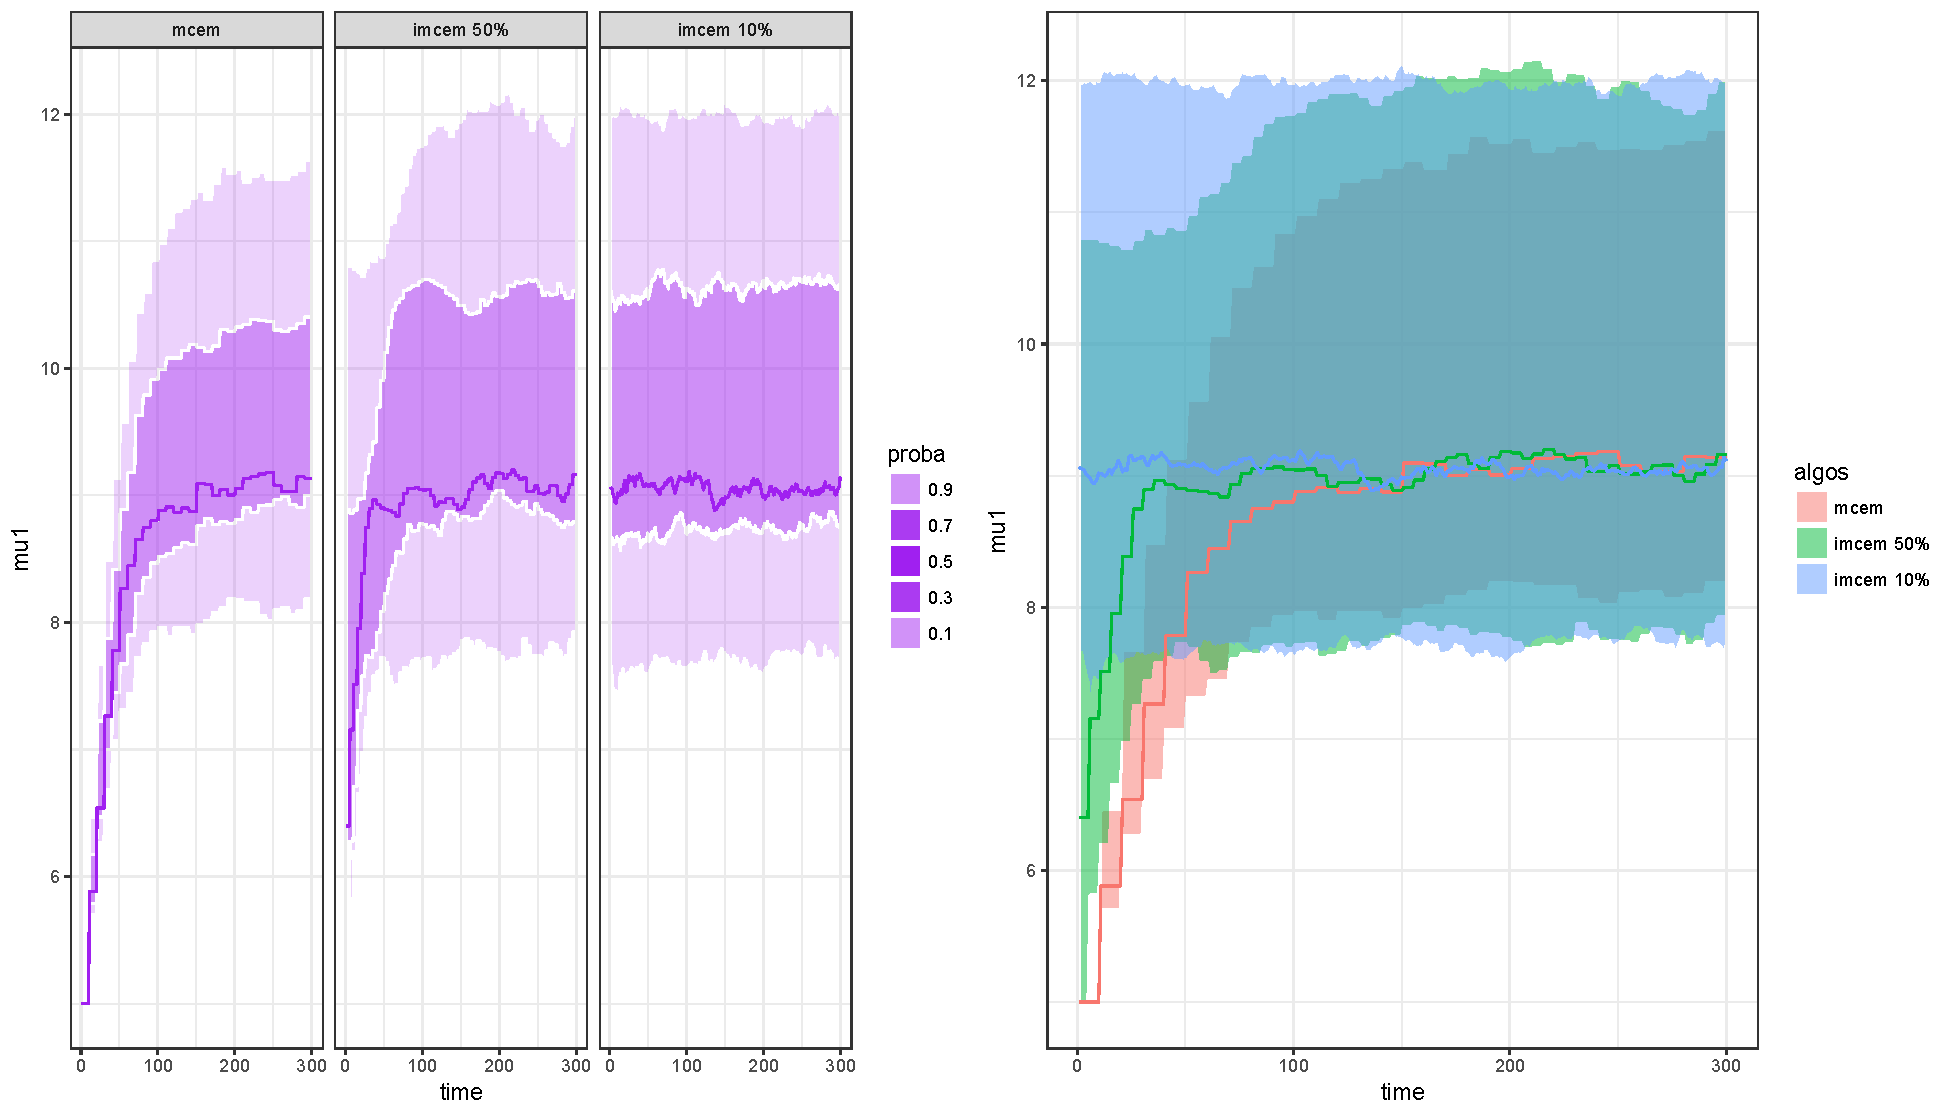
\includegraphics[width=25cm,height=10cm]{imcem_final.pdf}
\captionof{figure}{Incremental MCEM for 50 replicates}
\label{fig-dyn}
\end{center}\vspace{1cm}


\subsection{ISAEM on a PK-PD dataset}




We use an example used by P. Girard and F. Mentre for the symposium dedicated to Comparison of Algorithms Using Simulated Data Sets and Blind Analysis, that took place in Lyon, France, September 2004.\\
The dataset contains 100 individuals, each receiving 3 different doses:$(0, 10, 90)$, $(5, 25, 65)$ or $(0,20, 30)$. It was assumed that doses were given in a cross-over study with sufficient wash out period to avoid carry over. Responses $y_{ij}$ were simulated with the following pharmacodynamic model:
\begin{tcolorbox}[ams gather]
y_{ij} = E0_i + D_{ij} Emax_i/(D_{ij} + EC50_i) +\epsilon_{ij}
\end{tcolorbox}
Where $D_{ij}$ is the dose given to individual $i$ at time $t_j$ and the individual parameters $(E0_i,Emax_i,EC50_i)$ follow log normal distribution.


\begin{center}%\vspace{1cm}
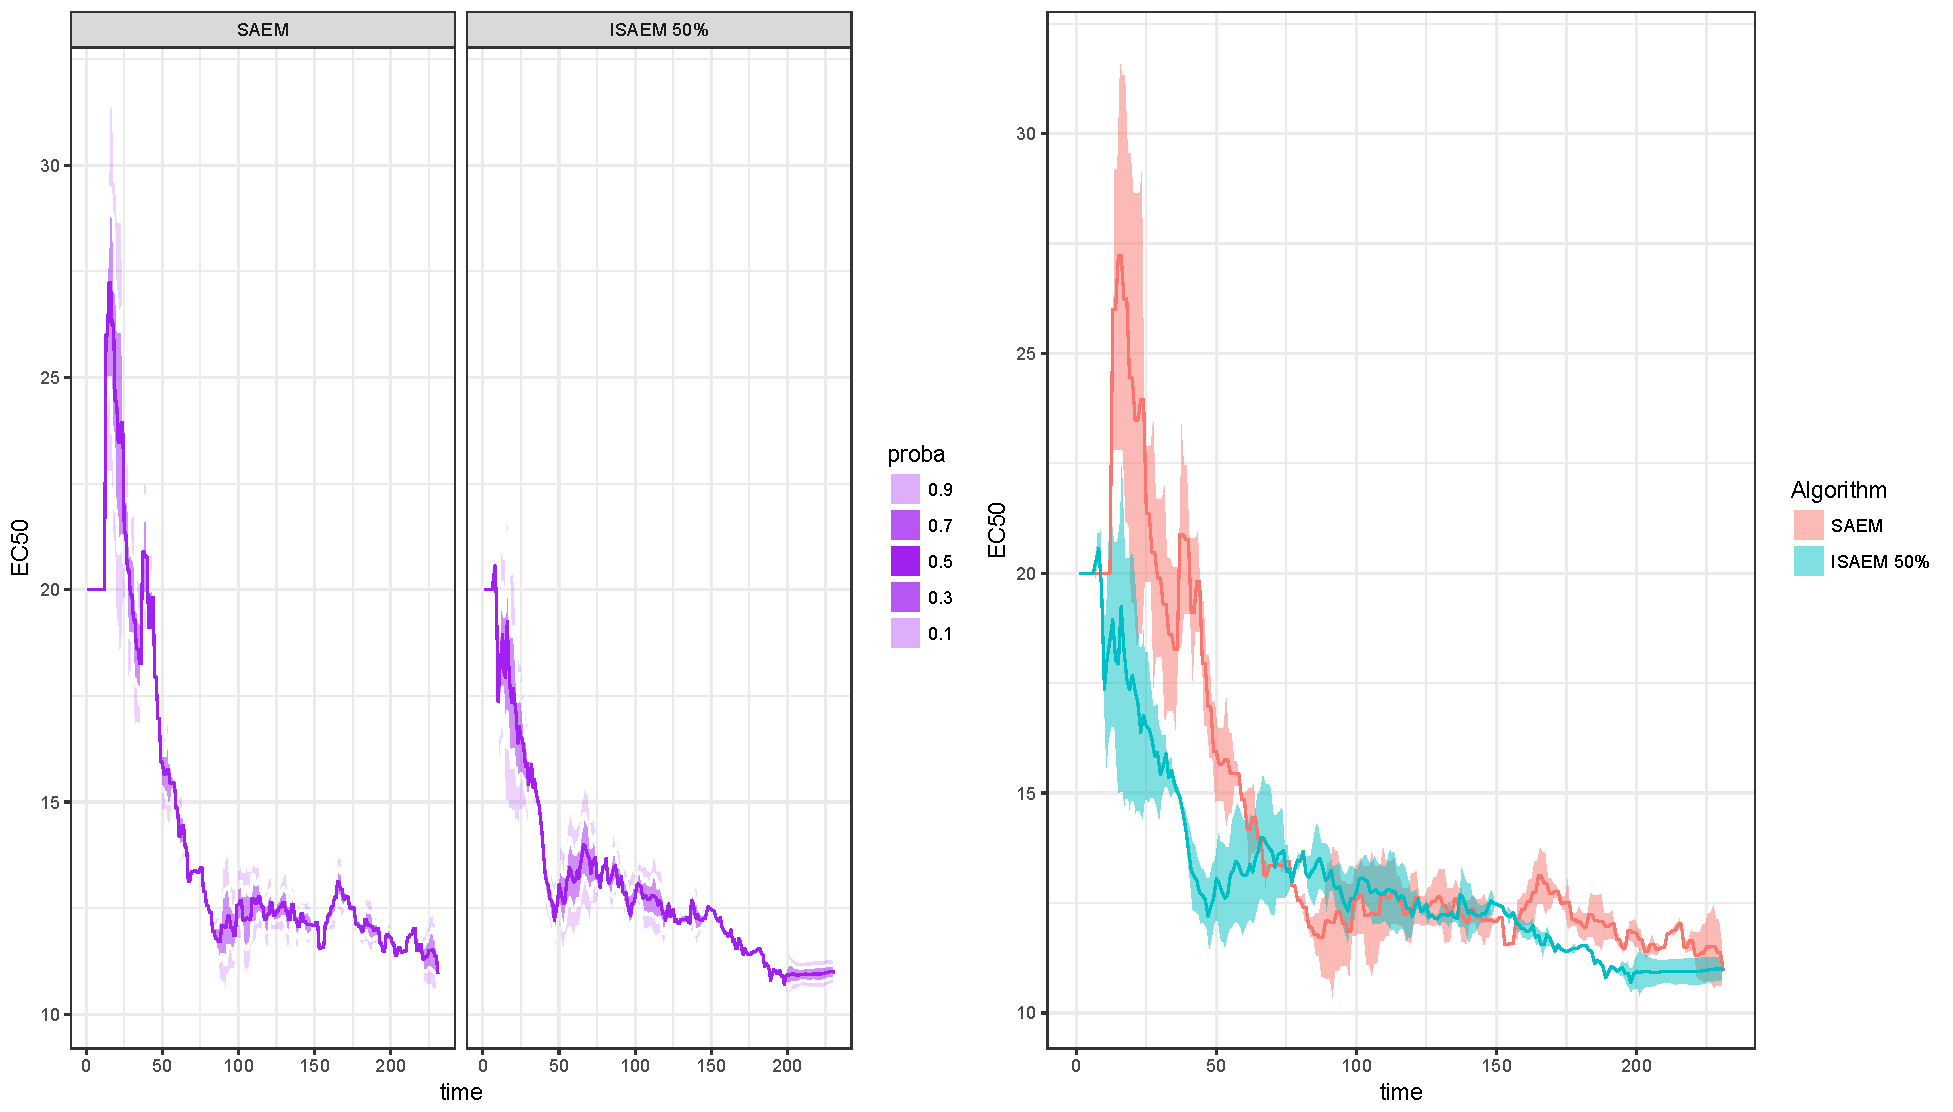
\includegraphics[width=25cm,height=10cm]{isaem_pd_final.pdf}
\captionof{figure}{Incremental SAEM for 50 replicates}
\label{fig-dyn}
\end{center}\vspace{1cm}

%\begin{center}\vspace{1cm}
%\includegraphics[width=0.8\linewidth]{resultats2}
%\captionof{figure}{Comparaison de la consommation de carburant avec et sans les commande optimisées }
%\end{center}\vspace{1cm}

%----------------------------------------------------------------------------------------
% CONCLUSIONS
%----------------------------------------------------------------------------------------

%\color{SaddleBrown} % SaddleBrown color for the conclusions to make them stand out
%\color{Navy}
%\vspace{1cm}
\section{Conclusion}
\color{Navy} % Navy color
We've shown convergence of incremental versions of the EM and stochastic EM algorithms but incremental variants also imply choice of the individuals at each iteration and the size of the number of individuals considered.\\
Even though Neal and Hinton showed that incremental EM was optimally fast when only one observation was considered at each iteration, stochastic versions behave differently. Current work is focusing on this aspect.


\color{DarkSlateGray} % Set the color back to DarkSlateGray for the rest of the content

%----------------------------------------------------------------------------------------
% FORTHCOMING RESEARCH
%----------------------------------------------------------------------------------------

%\section{Forthcoming Research}


 %----------------------------------------------------------------------------------------
% REFERENCES
%----------------------------------------------------------------------------------------


\small
\nocite{*} % Print all references regardless of whether they were cited in the poster or not
\bibliography{ref.bib}

%----------------------------------------------------------------------------------------
% ACKNOWLEDGEMENTS
%----------------------------------------------------------------------------------------

%\section*{Acknowledgements}

%\includegraphics[width=15cm]{opticlimb.png}\\


%----------------------------------------------------------------------------------------

\end{multicols}
\begin{center}
%
\includegraphics[width=10cm]{logo_x.jpg}
%
\includegraphics[width=10cm]{logo_inria.png}
%\includegraphics[width=15cm]{opticlimb.png}\\
\end{center}
\end{document}